\begin{frame}{Explicación gráfica del proceso I}
\centering
    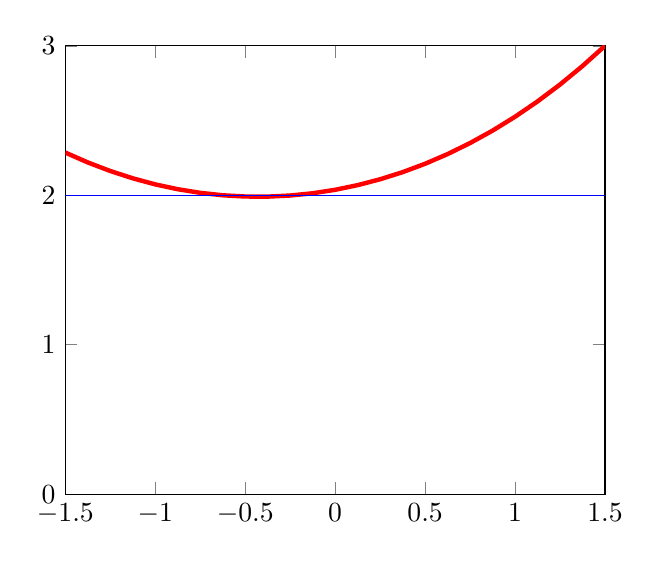
\begin{tikzpicture}
        \begin{axis}[
            xmin=-1.5,xmax=1.5,
            ymin=0,ymax=3]
            \addplot[domain=-1.5:1.5,draw=red,ultra thick]{1.99*cosh(((\x)+0.4285)/1.99)};           \addplot[domain=-1.5:1.5,draw=blue]{2};
        \end{axis}       
    \end{tikzpicture}
\end{frame}
\begin{frame}{Explicación gráfica del proceso II}
\centering
    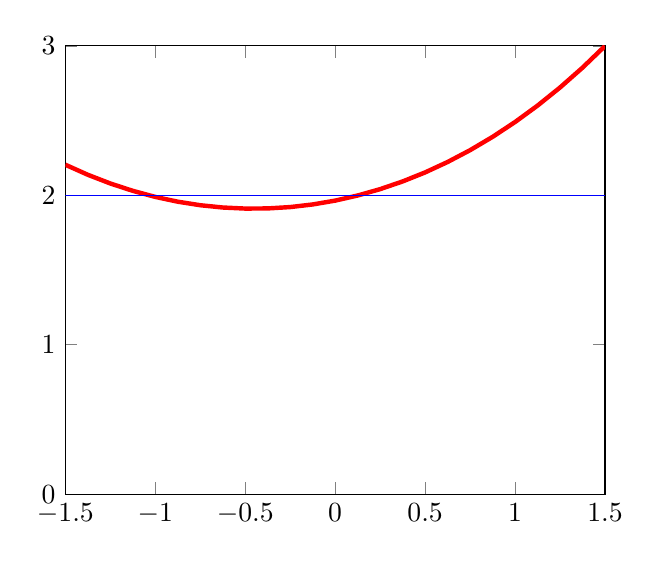
\begin{tikzpicture}
        \begin{axis}[
            xmin=-1.5,xmax=1.5,
            ymin=0,ymax=3]
            \addplot[domain=-1.5:1.5,draw=red,ultra thick]{1.91*cosh(((\x)+0.453)/1.91)};           \addplot[domain=-1.5:1.5,draw=blue]{2};
        \end{axis}       
    \end{tikzpicture}
\end{frame}
\begin{frame}{Explicación gráfica del proceso III}
\centering
    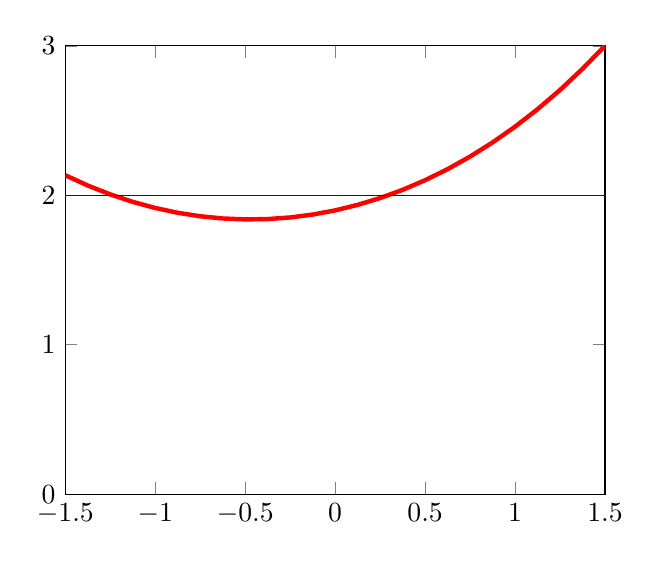
\begin{tikzpicture}
        \begin{axis}[
            xmin=-1.5,xmax=1.5,
            ymin=0,ymax=3]
            \addplot[domain=-1.5:1.5,draw=red,ultra thick]{1.838*cosh(((\x)+0.471)/1.838)};           \addplot[domain=-1.5:1.5,draw=blue]{2};
        \end{axis}       
    \end{tikzpicture}
\end{frame}
\begin{frame}{Explicación gráfica del proceso IV}
\centering
    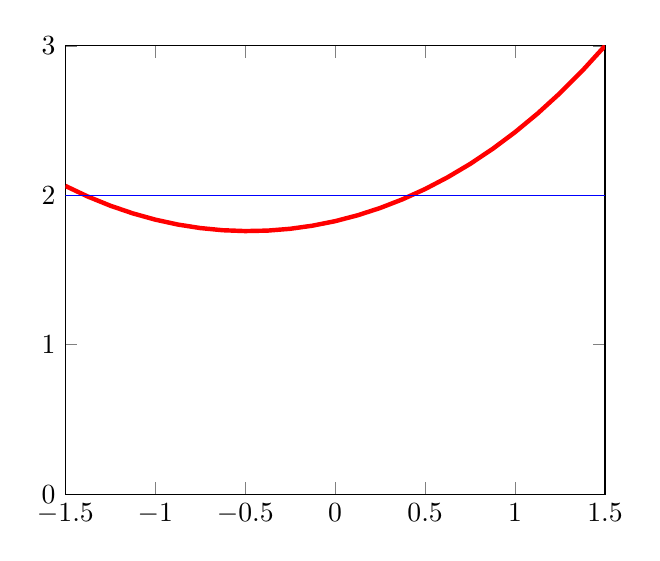
\begin{tikzpicture}
        \begin{axis}[
            xmin=-1.5,xmax=1.5,
            ymin=0,ymax=3]
            \addplot[domain=-1.5:1.5,draw=red,ultra thick]{1.76*cosh(((\x)+0.4824)/1.76)};           \addplot[domain=-1.5:1.5,draw=blue]{2};
        \end{axis}       
    \end{tikzpicture}
\end{frame}
\begin{frame}{Explicación gráfica del proceso V}
\centering
    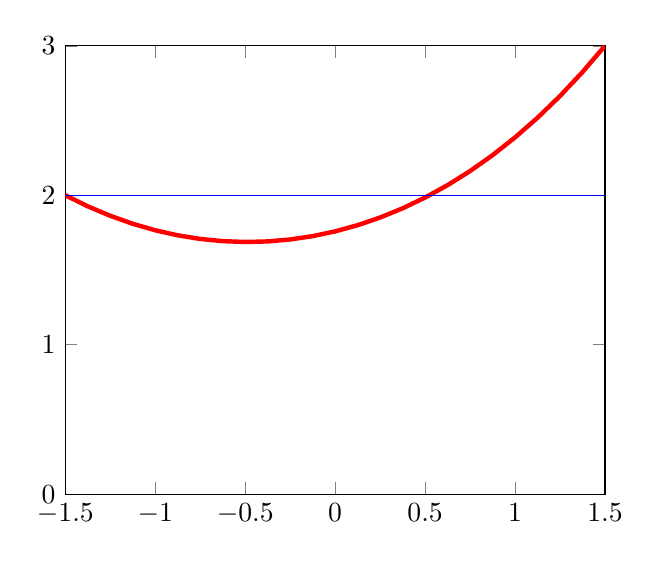
\begin{tikzpicture}
        \begin{axis}[
            xmin=-1.5,xmax=1.5,
            ymin=0,ymax=3]
            \addplot[domain=-1.5:1.5,draw=red,ultra thick]{1.6871*cosh(((\x)+0.4878)/1.6871)};           \addplot[domain=-1.5:1.5,draw=blue]{2};
        \end{axis}       
    \end{tikzpicture}
\end{frame}
